\subsection{Activation Functions}

\textcolor{blue}{Activation functions are XXXXXXXX}

\subsubsection{Why Non-linear}

\textcolor{blue}{Non-linear is necessary XXXXXXXXXX}

\subsubsection{Advancements}

\textcolor{green}{TODO: From step function to ?selu}

\subsubsection{Popular Activation Functions}

\textcolor{blue}{Activation functions can be grouped into two main categories -- smooth and not smooth. Smooth activation functions (such as sigmoid) are differentiable at every point along the function where as the other activation functions are not differentiable at every location (relu).}

% history
%differentiable everywhere, monotonic, and smooth.

\textcolor{blue}{linear (see above), }
	
\textcolor{blue}{tanh and sigmoid, (better because non-linear). however would saturate}

\textcolor{blue}{ReLu, better because \textcolor{red}{help prevent saturation}, but still have problems \textcolor{red}{can "die" at 0.} }

\textcolor{blue}{ELU fuctions. they prevent the "dying" problem by being \textcolor{red}{non-zero} but their main drawback is that they are more computationally expensive due to the calculation of the exponent.}

\paragraph{Smooth Non-linear}

\textcolor{blue}{The sigmoid\index{sigmoid} activation function}

% {{{act_smooth_sigmoid}}}
\begin{figure}
\centering
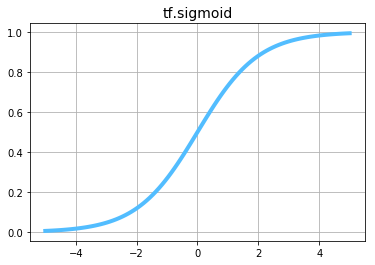
\includegraphics[width=0.65\textwidth]{./sync_imgs/act/smooth/sigmoid.png}
\label{fig:act_smooth_sigmoid}
\end{figure}

% {{{act_smooth_tangent}}}
\begin{figure}
\centering
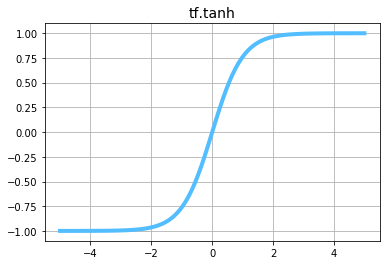
\includegraphics[width=0.65\textwidth]{./sync_imgs/act/smooth/tangent.png}
\label{fig:act_smooth_tangent}
\end{figure}

% {{{act_smooth_elu}}}
\begin{figure}
\centering
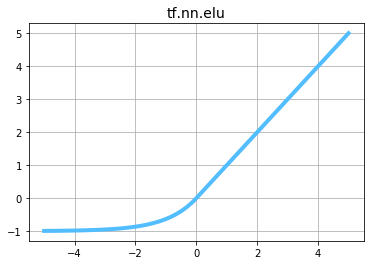
\includegraphics[width=0.65\textwidth]{./sync_imgs/act/smooth/elu.png}
\label{fig:act_smooth_elu}
\end{figure}

% {{{act_smooth_selu}}}
\begin{figure}
\centering
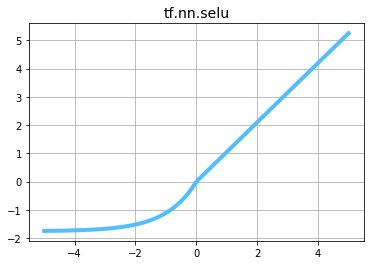
\includegraphics[width=0.65\textwidth]{./sync_imgs/act/smooth/selu.png}
\label{fig:act_smooth_selu}
\end{figure}

% {{{act_smooth_softplus}}}
\begin{figure}
\centering
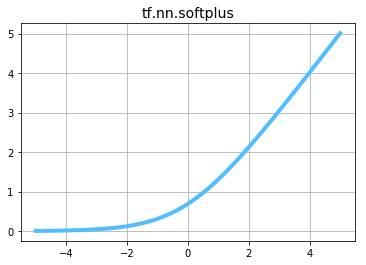
\includegraphics[width=0.65\textwidth]{./sync_imgs/act/smooth/softplus.png}
\label{fig:act_smooth_softplus}
\end{figure}

% {{{act_smooth_softsign}}}
\begin{figure}
\centering
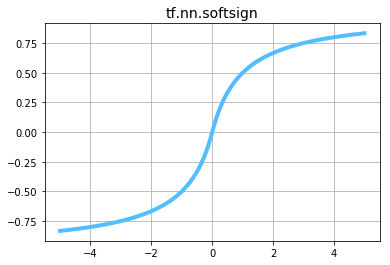
\includegraphics[width=0.65\textwidth]{./sync_imgs/act/smooth/softsign.png}
\label{fig:act_smooth_softsign}
\end{figure}


\paragraph{Not Smooth Non-linear}

% {{{act_notsmooth_relu}}}
\begin{figure}
\centering
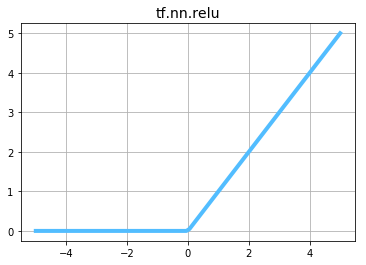
\includegraphics[width=0.65\textwidth]{./sync_imgs/act/notsmooth/relu.png}
\label{fig:act_notsmooth_relu}
\end{figure}

% {{{act_notsmooth_leakyrelu}}}
\begin{figure}
\centering
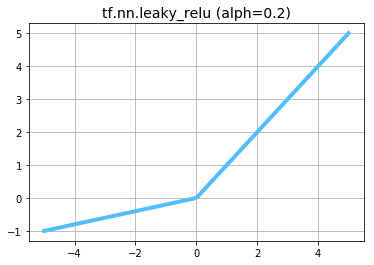
\includegraphics[width=0.65\textwidth]{./sync_imgs/act/notsmooth/leakyrelu.png}
\label{fig:act_notsmooth_leakyrelu}
\end{figure}

% {{{act_notsmooth_relu6}}}
\begin{figure}
\centering
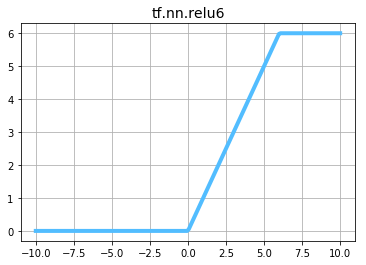
\includegraphics[width=0.65\textwidth]{./sync_imgs/act/notsmooth/relu6.png}
\label{fig:act_notsmooth_relu6}
\end{figure}

% {{{act_notsmooth_prelu}}}
\begin{figure}
\centering
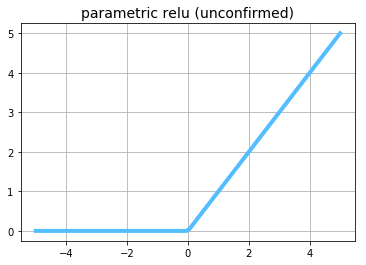
\includegraphics[width=0.65\textwidth]{./sync_imgs/act/notsmooth/prelu.png}
\label{fig:act_notsmooth_prelu}
\end{figure}

